\documentclass[
%journal=ancac3, % for ACS Nano
%journal=acbcct, % for ACS Chem. Biol.
journal=jacsat, % for undefined journal
manuscript=article]{achemso}
\usepackage[version=3]{mhchem} % Formula subscripts using \ce{}
\usepackage{tikz}
\usetikzlibrary{shapes,arrows}
\newcommand*{\mycommand}[1]{\texttt{\emph{#1}}}

\author{Tong He}
\affiliation[Simon Fraser University, Canada]
{Simon Fraser University, Canada}
\author{Marten Heidemeyer}
\affiliation[Simon Fraser University, Canada]
{Simon Fraser University, Canada}
%\altaffiliation{Simon Fraser University, Canada}
\author{Fuqiang Ban}
%\email{i.k.groupleader@unknown.uu}
\affiliation[Vancouver Prostate Center]
{Vancouver Prostate Center}
\author{Artem Cherkasov}
%\email{acherkasov@prostatecentre.com}
\affiliation[Vancouver Prostate Center]
{Vancouver Prostate Center}
\author{Martin Ester}
\affiliation[Simon Fraser University, Canada]
{Simon Fraser University, Canada}


\title[\texttt{achemso} demonstration]
{An accurate and confident prediction of drug-target binding affinity}
\usepackage{graphicx}

\begin{document}

\begin{abstract}
Computational prediction of the interaction between drugs and targets is a standing challenge in drug discovery. High performance on binary drug-target benchmark datasets was reported for a number of methods. As previously reported, a possible drawback of binary datasets is that missing values and non interacting drug-target pairs are not differentiated. In this paper we present a method that utilizes Continuous Conditional Random Fields (CCRF) to predict the continuous binding affinities of compounds and proteins and thus incorporates the whole interaction spectrum from true negative to true positive interactions in the learning phase. Additionally, our method computes a confidence score for each compound-protein pair in order to assess the confidence of the predicted affinity. We evaluate our model on three continuous drug-target dataset and we compare the performance of our model to a recently published similarity-based method for continuous binding affinity prediction. 

\end{abstract}

\section{1. Introduction}

Drug effects are caused by the interaction of drug compounds with proteins. Drug side effects occur when a drug compound is interacting with proteins other than its primary target. 
Knowledge about the interaction of drugs and targets (or more general drug candidate compounds and candidate target proteins) is therefore necessary in the process of drug development. Predicting the interaction between compounds and targets with computational methods is a hot topic in drug development because the in vitro validation of compound-protein interaction strengths is extremely costly and time consuming. A number of machine learning methods for large scale drug-target interaction prediction have been published so far and high accuracies in terms of AUC and AUPR were reported on binary drug target benchmark datasets. \citeauthor{ding2013similarity} reviews 6 methods, all of which were evaluated on binary datasets compiled from KEGG BRITE, BRENDA, SuperTarget, DrugBank, DCDB and ChEBI. These datasets record only validated interacting drug-target pairs and do not differentiate between missing measurements and non interacting drug target pairs. \citeauthor{ding2013similarity} and  \citeauthor{pahikkala2014toward} suggest that incorporating true negative interactions (observed non-interacting drug target pairs) could improve the performance of prediction models. Additionally, \citeauthor{pahikkala2014toward} suggests to build models that predict the continuous binding affinities of drugs and targets and present a kernel method for this task. In this study we present a new method for the task of predicting the continuous binding affinities between drugs and targets which is based on Continuous Conditional Random Fields. Binary Conditional Random Fields were previously applied by \citeauthor{yang2013drug} for the classification task of predicting if a drug target pair is interacting or not. We evaluate our model on four datasets of different sparsity and compare our model to the kernel method presented in \citeauthor{pahikkala2014toward} 


\section{Models and Method}

\subsection{Predictive Model}
Conditional Random Fields are a type of Markov Network that encode a conditional distribution $P(Y|X)$, where $Y$ is a set of target variables and $X$ is a set of observed variables. For the task of drug target interaction prediction, the vector $Y$ stands for the drug-target binding affinities that we wish to predict and the vector $X$ stands for a first prediction of the binding affinity. We utilized the CRF notation to integrate drug and target similarity matrices to improve the initial prediction $X$. In the used CRF model, the probability of a vector $Y$ given the initial prediction $X$ and a similarity score for all drug-target pairs is defined as follows:
\begin{center}
$P(Y|X) = \frac{1}{Z}exp(\alpha\sum\limits_{i}f(y_i,X_i)+\beta\sum\limits_{i,j}g(y_i,y_j))$
\end{center}
Here, the term $\alpha\sum\limits_{i}f(y_i,X_i)$ penalizes the difference of the prediction from the initial prediction and the term $\beta\sum\limits_{i,j}g(y_i,y_j)$ penalizes the difference of two similar drug-target pairs. Formally, $f$ is defined as $f(y_i,X_i) = -(y_i-X_i)^2$ and $g$ is defined as $g(y_i, y_j, X_i) = -\frac{1}{2}S_{i,j}(y_i-y_j)^2$. Figure 1 illustrates the graphical structure of the CRF.


\begin{figure}
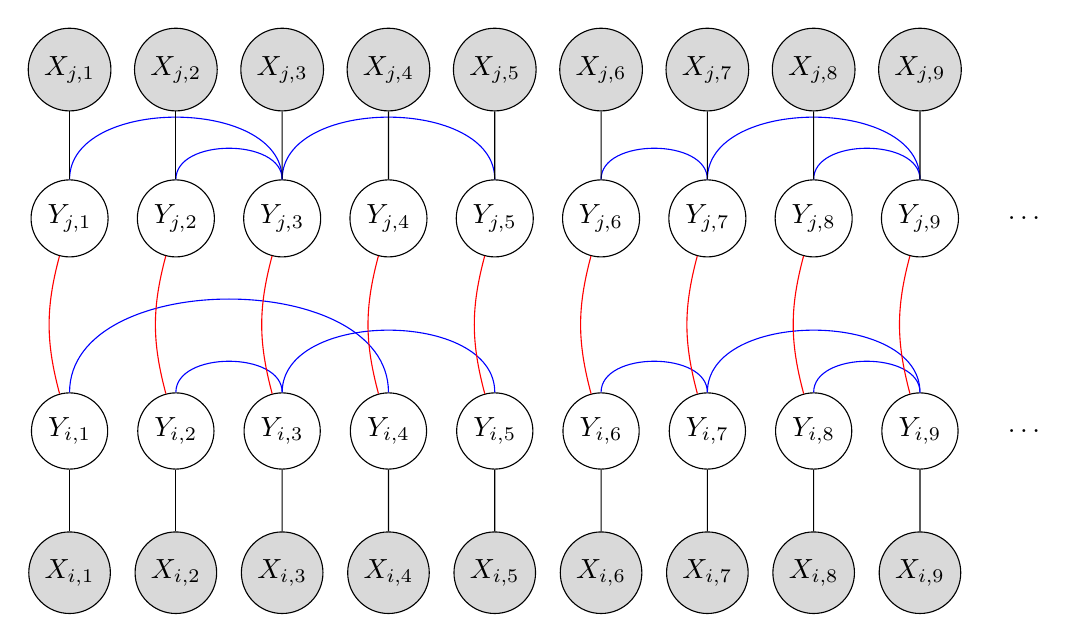
\begin{tikzpicture}[scale=.9]
\tikzstyle{every node} = [draw, shape=circle]
\node (a) at (0, 0) {$Y_{i, 1}$};
\node (b) at (1.5, 0) {$Y_{i, 2}$};
\node (c) at (3, 0) {$Y_{i, 3}$};
\node (d) at (4.5, 0) {$Y_{i, 4}$};
\node (e) at (6, 0) {$Y_{i, 5}$};
\node (f) at (7.5, 0) {$Y_{i, 6}$};
\node (g) at (9, 0) {$Y_{i, 7}$};
\node (h) at (10.5, 0) {$Y_{i, 8}$};
\node (i) at (12, 0) {$Y_{i, 9}$};
\node [draw=none] (j) at (13.5,0) {$\dots$};
\draw [-, draw=blue] (a) to  [out=90,in=90] (d);
\draw [-, draw=blue] (c) to  [out=90,in=90] (b);
\draw [-, draw=blue] (c) to  [out=90,in=90] (e);
\draw [-, draw=blue] (h) to  [out=90,in=90] (i);
\draw [-, draw=blue] (g) to  [out=90,in=90] (f);
\draw [-, draw=blue] (g) to  [out=90,in=90] (i);

\node [fill=gray!30 ](x1) at (0, -2) {$X_{i, 1}$};
\node [fill=gray!30 ](x2) at (1.5, -2) {$X_{i, 2}$};
\node [fill=gray!30 ](x3) at (3, -2) {$X_{i, 3}$};
\node [fill=gray!30 ](x4) at (4.5, -2) {$X_{i, 4}$};
\node [fill=gray!30 ](x5) at (6, -2) {$X_{i, 5}$};
\node [fill=gray!30 ](x6) at (7.5, -2) {$X_{i, 6}$};
\node [fill=gray!30 ](x7) at (9, -2) {$X_{i, 7}$};
\node [fill=gray!30 ](x8) at (10.5, -2) {$X_{i, 8}$};
\node [fill=gray!30 ](x9) at (12, -2) {$X_{i,9}$};
\draw [-] (a) to  [out=270,in=90] (x1);
\draw [-] (b) to  [out=270,in=90] (x2);
\draw [-] (c) to  [out=270,in=90] (x3);
\draw [-] (d) to  [out=270,in=90] (x4);
\draw [-] (e) to  [out=270,in=90] (x5);
\draw [-] (f) to  [out=270,in=90] (x6);
\draw [-] (g) to  [out=270,in=90] (x7);
\draw [-] (h) to  [out=270,in=90] (x8);
\draw [-] (i) to  [out=270,in=90] (x9);

\node (a2) at (0, 3) {$Y_{j, 1}$};
\node (b2) at (1.5, 3) {$Y_{j, 2}$};
\node (c2) at (3, 3) {$Y_{j, 3}$};
\node (d2) at (4.5, 3) {$Y_{j, 4}$};
\node (e2) at (6, 3) {$Y_{j, 5}$};
\node (f2) at (7.5, 3) {$Y_{j, 6}$};
\node (g2) at (9, 3) {$Y_{j, 7}$};
\node (h2) at (10.5,3) {$Y_{j, 8}$};
\node (i2) at (12, 3) {$Y_{j, 9}$};
\node [draw=none] (j) at (13.5,3) {$\dots$};
\draw [-, draw=blue] (a2) to  [out=90,in=90] (c2);
\draw [-, draw=blue] (c2) to  [out=90,in=90] (b2);
\draw [-, draw=blue] (c2) to  [out=90,in=90] (e2);
\draw [-, draw=blue] (h2) to  [out=90,in=90] (i2);
\draw [-, draw=blue] (g2) to  [out=90,in=90] (f2);
\draw [-, draw=blue] (g2) to  [out=90,in=90] (i2);

\node [fill=gray!30 ](x11) at (0, 5.1) {$X_{j, 1}$};
\node [fill=gray!30 ](x21) at (1.5, 5.1) {$X_{j, 2}$};
\node [fill=gray!30 ](x31) at (3, 5.1) {$X_{j, 3}$};
\node [fill=gray!30 ](x41) at (4.5, 5.1) {$X_{j, 4}$};
\node [fill=gray!30 ](x51) at (6, 5.1) {$X_{j, 5}$};
\node [fill=gray!30 ](x61) at (7.5, 5.1) {$X_{j, 6}$};
\node [fill=gray!30 ](x71) at (9, 5.1) {$X_{j, 7}$};
\node [fill=gray!30 ](x81) at (10.5, 5.1) {$X_{j, 8}$};
\node [fill=gray!30 ](x91) at (12, 5.1) {$X_{j,9}$};
\draw [-] (a2) to  [out=90,in=270] (x11);
\draw [-] (b2) to  [out=90,in=270] (x21);
\draw [-] (c2) to  [out=90,in=270] (x31);
\draw [-] (d2) to  [out=90,in=270] (x41);
\draw [-] (e2) to  [out=90,in=270] (x51);
\draw [-] (f2) to  [out=90,in=270] (x61);
\draw [-] (g2) to  [out=90,in=270] (x71);
\draw [-] (h2) to  [out=90,in=270] (x81);
\draw [-] (i2) to  [out=90,in=270] (x91);


\draw [-, draw=red] (a2) to  [out=255,in=105] (a);
\draw [-, draw=red] (b2) to  [out=255,in=105] (b);
\draw [-, draw=red] (c2) to  [out=255,in=105] (c);
\draw [-, draw=red] (d2) to  [out=255,in=105] (d);
\draw [-, draw=red] (e2) to  [out=255,in=105] (e);
\draw [-, draw=red] (f2) to  [out=255,in=105] (f);
\draw [-, draw=red] (g2) to  [out=255,in=105] (g);
\draw [-, draw=red] (h2) to  [out=255,in=105] (h);
\draw [-, draw=red] (i2) to  [out=255,in=105] (i);
\end{tikzpicture}
\caption{CRF over drugs $d_i$ and $d_j$ and targets $t_i,\dots,t_9$:  The intuition behind the CRF is to predict binding affinities, s.th. (a) the predictions are not too far from the predicted affinity of Matrix-Factorization ($X$), (b) the predicted binding strengths of similar targets (blue edges) are similar and (c) the predicted  binding strengths of similar drugs (red edges) are similar. The importance of the first prediction $X$, and the drug- and target similarities is weighted with parameters $\alpha$, $\beta_1$ and $\beta_2$ which are learned in the training step. In order to keep the inference step tractable, the number of nodes in the CRF is kept low by clustering the drugs (targets) and learn separate parameters for each drug cluster (target cluster). The above example illustrates a CRF over the two similar drugs $d_i$ and $d_j$. In the experiments on the datasets that are reported in this paper, CRFs were build for single drugs, single targets, drug clusters and target clusters. When a CRF was build for a drug-cluster (target-cluster), it consisted of nodes for the respective drugs (targets) and all targets (drugs). Suppose a dataset with 3000 drugs and 400 targets: A CRF over a drug cluster with 10 drugs, consists of 10 $\times$ 400  = 4000 nodes and the matrix that needs to be inverted in the inference step is of size $16.000.000 \times 16.000.000$. Thus the number of drugs (targets) in the clusters need to be kept rather small.
}
\end{figure}

\subsubsection{Parameter Learning}

\subsubsection{Inference}

\subsection{Experimental Settings}
The performance of the model was evaluated by 5 fold Cross Validation on the drug-target pairs. Therefore the drug-target matrix was randomly partitioned into 5 parts, of which each was removed in turn from the training set and used as test data. The approach corresponds to the use case where it is the aim to predict the interaction affinities for the missing drug-target pairs where both, the drug and the target, have been encountered in the training set.



\subsection{Model Evaluation}

\subsubsection{Evaluation Datasets}
In addition to the \textit{Davis} and \textit{Metz} (\citeauthor{davis2011comprehensive} and \citeauthor{metz2011navigating}) that were already used in the study by \citeauthor{pahikkala2014toward} two sparser datasets (Kiba 1 and Kiba 2) were compiled from the kinase dataset that was originally compiled from a number of sources by \citeauthor{doi:10.1021/ci400709d} This dataset contains originally 52.498 compounds and 467 targets. The evaluation dataset \mbox{Kiba 1} was obtained by removing all drugs and targets with less than 10 observations from this dataset. A fourth evaluation dataset (Kiba 2) with the highest sparsity was created by sampling half of the observations from dataset \mbox{Kiba 1}.
\begin{table}[]
\centering
\begin{tabular}{l c c c}
Dataset & Drugs & Targets & Density \\
\hline
Davis & 68 & 442 & 100\%\\
Metz & 1421 & 156 & 42.1\%\\
Kiba 1 & 2116 & 229 & 24.4\%\\
Kiba 2 & 2116& 229 & 12.21\%\\
\end{tabular}
\caption{statistics of the used evaluation datasets.}
\label{dataset_stats}
\end{table}

\subsubsection{Evaluation Metrics}
To evaluate the continuous predictions, we used the concordance index (CI) as an evaluation metric for the prediction accuray as suggested by \citeauthor{pahikkala2014toward}. As described by \citeauthor{pahikkala2014toward}, the CI over a set of paired data is the probability that the predictions for two randomly drawn drug-target pairs with different label values are in the correct order and is defined as:
\begin{center}
$CI = \frac{1}{Z}\sum\limits_{y_i> y_j}h(f_i-f_j)$
\end{center}
where $h(u)$ is the step function, returning 1.0, 0.5 and 0.0 for $u>0$, $u=0$ and $u<0$ respectively and $f_i$ is the prediction for the larger binding affinity $y_i$ and $f_j$ is the prediction for the smaller binding affinity $y_j$.

\subsubsection{Binary vs. Continuous Prediction}

\section{Results}
\begin{center}
\begin{tabular}{l | c}
Dataset & CI \\
\hline
Davis &
\begin{tabular}{c c}
KronRLS & CCRF \\ \hline
\begin{tabular}{c|c|c}
2D & \textbf{88.3} & \\ \hline
$\delta$ &  &\\ \hline
 & SW & $\delta$\\
\end{tabular} & 
\begin{tabular}{c|c|c} 
2D &  87.1& \\ \hline
$\delta$ &  & \\ \hline
& SW & $\delta$ \\
\end{tabular} 
\end{tabular} \\
Metz & 
\begin{tabular}{c c}
KronRLS & CCRF \\ \hline
\begin{tabular}{c|c|c}
2D & 79.3 &   \\ \hline
$\delta$ &  & \\ \hline
 & SW & $\delta$\\
\end{tabular} & 
\begin{tabular}{c|c|c} 
2D & \textbf{81.8} & \\ \hline
$\delta$ &  & \\ \hline
& SW & $\delta$ \\
\end{tabular} 
\end{tabular} \\
Kiba 1& 
\begin{tabular}{c c}
KronRLS & CCRF \\ \hline
\begin{tabular}{c|c|c}
2D & 78.3 & \\ \hline
$\delta$ & & \\ \hline
 & SW & $\delta$\\
\end{tabular} & 
\begin{tabular}{c|c|c} 
2D & \textbf{81.9} & \\ \hline
$\delta$ & & \\ \hline
& SW & $\delta$ \\
\end{tabular} 
\end{tabular}\\
Kiba 2& 
\begin{tabular}{c c}
KronRLS & CCRF \\ \hline
\begin{tabular}{c|c|c}
2D & 76.1 & \\ \hline
$\delta$ & & \\ \hline
 & SW & $\delta$\\
\end{tabular} & 
\begin{tabular}{c|c|c} 
2D & \textbf{78.7}& \\ \hline
$\delta$ & & \\ \hline
& SW & $\delta$ \\
\end{tabular} 
\end{tabular}\\
\end{tabular}
\end{center}


\begin{center}
\begin{tabular}{l | c}
Dataset & AUC\\
\hline
Davis & 
\begin{tabular}{c c}
KronRLS & CCRF \\ \hline
\begin{tabular}{c|c|c}
2D & \textbf{0.952} & 0.729\\ \hline
$\delta$ & 0.927 & \\ \hline
 & SW & $\delta$\\
\end{tabular} & 
\begin{tabular}{c|c|c} 
2D & 0.937 & 0.873\\ \hline
$\delta$ & 0.933 &  0.869\\ \hline
 & SW & $\delta$ \\
\end{tabular} 
\end{tabular}  
 \\
Metz & 
\begin{tabular}{c c}
KronRLS & CCRF \\ \hline
\begin{tabular}{c|c|c}
2D & 0.934 & 0.868 \\ \hline
$\delta$ & 0.846 & \\ \hline
 & SW & $\delta$\\
\end{tabular} & 
\begin{tabular}{c|c|c} 
2D & \textbf{0.947} & \\ \hline
$\delta$ &  & 0.885\\ \hline
 & SW & $\delta$ \\
\end{tabular} 
\end{tabular} \\
Kiba 1& 
\begin{tabular}{c c}
KronRLS & CCRF \\ \hline
\begin{tabular}{c|c|c}
2D & \textbf{0.908} & \\ \hline
$\delta$ & & \\ \hline
 & SW & $\delta$\\
\end{tabular} & 
\begin{tabular}{c|c|c} 
2D & 0.87 & \\ \hline
$\delta$ & &0.833 \\ \hline
 & SW & $\delta$ \\
\end{tabular} 
\end{tabular}  \\
Kiba 2& 
\begin{tabular}{c c}
KronRLS & CCRF \\ \hline
\begin{tabular}{c|c|c}
2D & 0.908 & \\ \hline
$\delta$ & & \\ \hline
 & SW & $\delta$\\
\end{tabular} & 
\begin{tabular}{c|c|c} 
2D & 0.87& \\ \hline
$\delta$ & &0.833 \\ \hline
 & SW & $\delta$ \\
\end{tabular} 
\end{tabular}  \\
\end{tabular}\\
\vspace{1cm}
\begin{tabular}{l | c}
Dataset & AUPR \\
\hline
Davis &
\begin{tabular}{c c}
KronRLS & CCRF \\ \hline
\begin{tabular}{c|c|c}
2D & \textbf{0.67} & 0. 279\\ \hline
$\delta$ & 0.649 &\\ \hline
 & SW & $\delta$\\
\end{tabular} & 
\begin{tabular}{c|c|c} 
2D & 0.63 & \\ \hline
$\delta$ &  & \\ \hline
 & SW & $\delta$ \\
\end{tabular} 
\end{tabular} \\
Metz & 
\begin{tabular}{c c}
KronRLS & CCRF \\ \hline
\begin{tabular}{c|c|c}
2D &  0.572 &  0.44 \\ \hline
$\delta$ & 0.28 & \\ \hline
 & SW & $\delta$\\
\end{tabular} & 
\begin{tabular}{c|c|c} 
2D & \textbf{0.577} & 0.515\\ \hline
$\delta$ & 0.431 & 0.331\\ \hline
 & SW & $\delta$ \\
\end{tabular} 
\end{tabular} \\
Kiba 1& 
\begin{tabular}{c c}
KronRLS & CCRF \\ \hline
\begin{tabular}{c|c|c}
2D & \textbf{0.754} & \\ \hline
$\delta$ & & \\ \hline
 & SW & $\delta$\\
\end{tabular} & 
\begin{tabular}{c|c|c} 
2D & 0.736 & \\ \hline
$\delta$ & & \\ \hline
 & SW & $\delta$ \\
\end{tabular} \\
\end{tabular}\\
Kiba 2& 
\begin{tabular}{c c}
KronRLS & CCRF \\ \hline
\begin{tabular}{c|c|c}
2D &  & \\ \hline
$\delta$ & & \\ \hline
 & SW & $\delta$\\
\end{tabular} & 
\begin{tabular}{c|c|c} 
2D & & \\ \hline
$\delta$ & & \\ \hline
 & SW & $\delta$ \\
\end{tabular} \\
\end{tabular}\\
\end{tabular}\\
\vspace{1cm}
\end{center}

\bibliographystyle{plain}
\bibliography{bibliography} 

\end{document}